% !TeX root = ../thesis.tex

\chapter{随机传值进程模型}

由于Uniform Approach是模型无关的概率扩展方法,
我们可以使用该方法概率化扩展其他的进程模型。
本章会对传值进程模型进行概率化扩展。
传值进程模型是经典的进程模型,
在Milner的Communication and Concurrency一书中,
也是使用传值的通信并发模型——消息的发送者、接受者和通信媒介——引入并发和通信的概念。
我们选择传值进程模型的一种定义——The Value-Passing Calculus进行扩展。

\section{传值进程模型}
传值进程模型(Value-Passing Calculus)是一种
可以将某个域中的值作为通信的内容,
并且可以在特定逻辑条件执行某个动作的并发进程模型。
一个经典的例子是Milner书中的一单元缓冲区,它可以接受、储存、发送消息:
\begin{align*}
   C&\stackrel{def}{=}in(x).C'(x)\\
   C'(x)&\stackrel{def}{=}\overline{out}(x).C
\end{align*}
更“普遍”的传值进程模型也可以对输入进行逻辑判定,
根据特定的“条件”执行特定的“动作”,
通过输入控制进程的执行。我们以进程$A(x)$为例:
$$A(x)=\textrm{if }\varphi(x)\textrm{ then }\overline{a}(f(t))\textrm{ else }B(x)$$
$A(x)$在满足条件$\varphi(x)$时会通过通道$a$输出函数$f(t)$的值,
其中$t$可能是$x$的函数,也可能与$x$无关;若不满足$\varphi(x)$,则执行程序$B(x)$。

传值进程模型赋予了进程传递数据的能力,
我们可以通过进程之间传递的数据来控制进程的执行和进程间的交互,
这种控制能力显著的增强了并发进程模型的表达能力,拓宽了应用场景。
在网络通信中,各种通信协议通过在主机间传值进而控制主机的行为,
通信协议的过程就可以被抽象为传值进程模型,
支持并发的编程语言也可以被解释为传值进程模型,如Erlang。
很多通过传值,计算解决的现实问题也都可以抽象为传值进程模型。


\subsection{The Value-Passing Calculus}\label{ch:vpc}
对传值进程模型的研究很多都会依赖一个“神域”,
这个“神域”提供条件的判定,函数的计算和变量的取值范围。
如在执行$A(x)$时,我们会将$\varphi(x)$传给“神域”,
“神域”判定是否满足条件,并将判定结果返回给我们,
同样的,我们也会将$f(t)$传给“神域”,“神域”帮我们计算这个函数,并将结果返回给我们。
“神域”通常不包括在传值进程模型中,且通常是未定义的,或只在特定场景下定义。
由于“神域”的存在,对于这些传值进程模型表达能力的衡量变得十分困难,
Fu在The Value-Passing Calculus中取缔了“神域”的概念,
提出了一个封闭的传值进程模型。

The Value-Passing Calculus中的传值进程模型$\mathbb{VPC}_{\mathsf{Th}}$
的语法可以表示为:
\begin{equation}\label{eq:vpc}
   T:=\sum_{i\in I}\varphi_i a(x).T_i|\sum_{i\in I}\varphi_i\overline{a}(t_i).T_i|T|T'|(c)T|\varphi T|!a(x).T|!\overline{a}(t).T
\end{equation}
其中$T$是一个$\mathbb{VPC}_{\mathsf{Th}}$项,$\mathsf{Th}$是可判定的逻辑,
$\varphi_i$是一个布尔表达式,可以通过$\mathsf{Th}$证明或证伪,
若$\mathsf{Th}$可以给出$\varphi_i$的一个证明,记为$\mathsf{Th}\vdash \varphi_i$。
$a(x)$是一个输入前缀,$\overline{a}(t_i)$是一个输出前缀,
我们可以用$\sum_{i\in I}\varphi_i\lambda_i.T_i$来表示$\sum_{i\in I}\varphi_i a(x).T_i$或$\sum_{i\in I}\varphi_i \overline{a}(t).T_i$。
$!a(x).T$和$!\overline{a}(t).T$对应递归操作,$\mu X.E$可以表示为
$(c)(E\{c(z).0/X\}|!\overline{c}(r).E\{c(z).0/X\})$。
其余的表达与第一章CCS语法定义的解释相同。

The Value-Passing Calculus提出了两种转移语义的描述:具体语义(Concrete Semantics)和符号语义(Symbolic Semantics)。
后文我们只用到了符号语义,因此我们忽略具体语义的相关内容。

$\mathbb{VPC}_{\mathsf{Th}}$的符号语义如图~\ref{fig_vpc}所示。

\begin{figure}[!htbp]
   \small
   \centering
   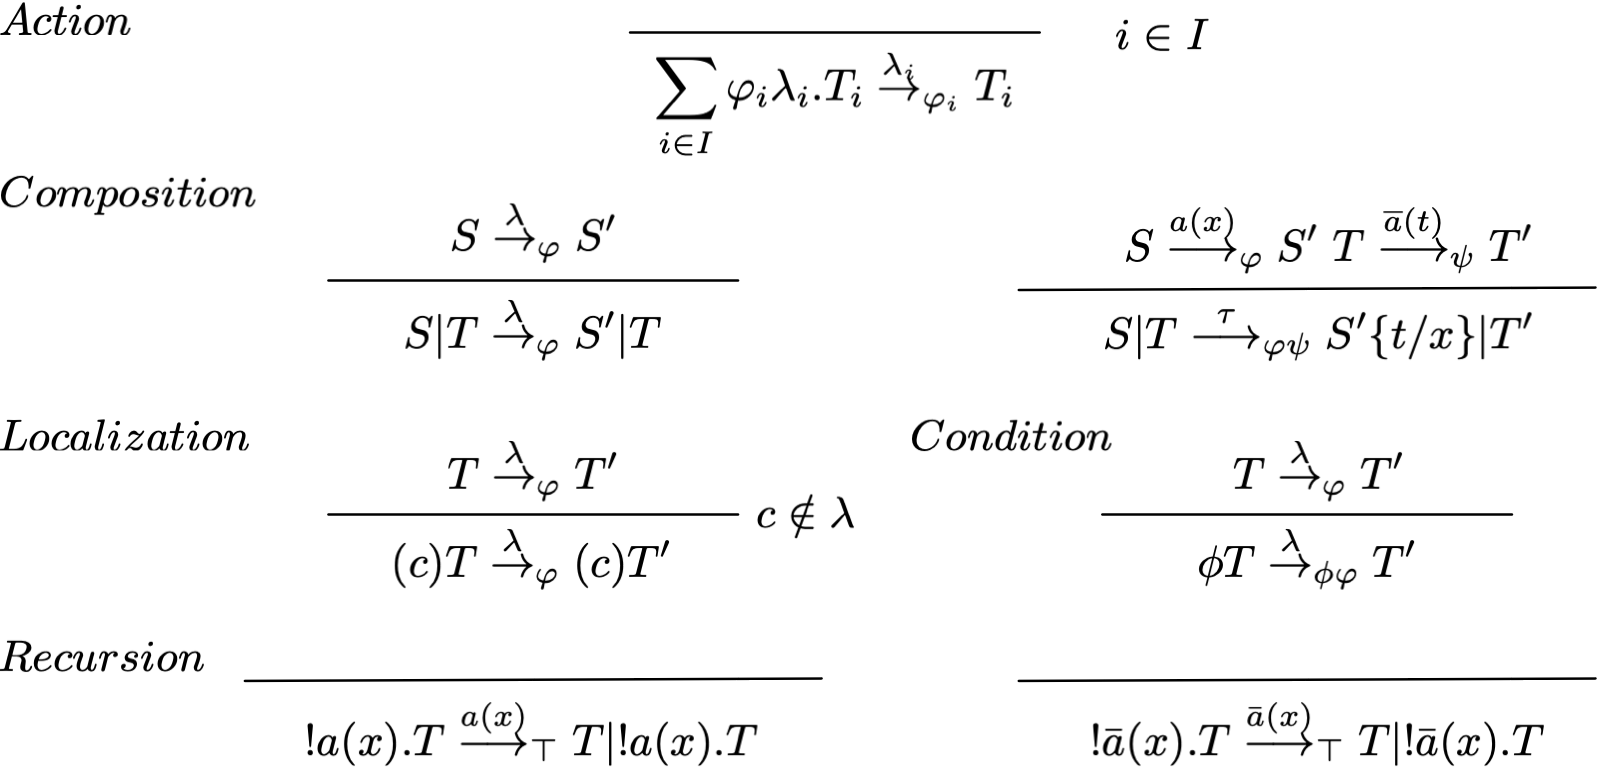
\includegraphics[width=13cm]{../figure/vpc.png}
    \caption[]{$\mathbb{VPC}_{\mathsf{Th}}$的符号语义规则}
    \label{fig_vpc}
\end{figure}
其中,$T=\varphi \lambda.T'$在$\varphi$条件下执行$\lambda$动作到达$T'$状态,
在符号语义下可以写作$T\stackrel{\lambda}{\rightarrow}_{\varphi}T'$。
符号语义中的动作集合$Act=\{a(x),\overline{a}(t)| a\in Chan, x\in \mathsf{V}_{\Sigma}, t\in \mathsf{T}_{\Sigma}\}\cup \{\tau\}$,
$Act$中的元素可以用$\lambda$表示,其中$\mathsf{V}_{\Sigma},\mathsf{T}_{\Sigma}$为可判定逻辑$\mathsf{Th}$中变量的集合和项的集合[引用]。

The Value-Passing Calculus使用可判定的一阶理论判定条件并
提出了一个图灵完备的数值系统(Numeric System)作为底层模型来实现可计算的函数。
通过这两种方式,将Value-Passing Calculus从“神域”中解放出来。

\subsection{If Then Else语法符号化}
进程$A(x)$中出现了If Then Else语法,
If Then Else语法实现的分支控制在编程中也是非常重要的组成部分。
在Milner的Communication and Concurrency一书中也多次使用If Then Else语法,
然而在CCS的定义中,我们无法通过CCS代理的语法规则来实现这种分支控制;
书中对分支控制的使用,如第五章(Bisimulation and Observation Equivalence)中对JobShop的建模,
也比较随意,没有严格的定义也没有判断If条件的可判定性。
在Fu的The Value-Passing Calculus中,
规定了If条件是通过一阶理论$\mathsf{Th}$可判定的布尔表达式,
并说明$\textrm{if }\varphi\textrm{ then }S\textrm{ else }T$
可以被定义为$\varphi S|\urcorner \varphi T$。
以下推论依据The Value-Passing Calculus中对If Then Else语法的定义和$\mathbb{VPC}_{\mathsf{Th}}$的Proof System,
给出If Then Else的变体的符号化定义,在本文的后续章节会统一使用这些符号。

以下推论中$S,T\in \mathcal{T}_{\mathbb{VPC}_\mathsf{Th}}$。
\begin{corollary} 
   $\varphi 0 = 0$
\end{corollary}
\begin{proof}
   $\varphi 0 = \varphi 0 + 0 = \varphi 0 + \top 0 = \varphi 0 + (\varphi \vee \urcorner \varphi)0 = \varphi 0 + \varphi 0 + \urcorner \varphi 0 = \varphi 0 + \urcorner \varphi 0 = (\varphi \vee \urcorner \varphi)0 = \top 0 = 0$
\end{proof}
\begin{corollary}
   $\varphi T = (\varphi T\mid \urcorner \varphi 0)$
\end{corollary}
\begin{proof}
   $\varphi T = (\varphi T\mid 0) = (\varphi T\mid \urcorner \varphi 0)$
\end{proof}
\begin{corollary}
   $S=\urcorner\varphi \varphi T$,则$S=0$。
\end{corollary}
\begin{proof}
   $S=\urcorner\varphi \varphi T = (\urcorner\varphi\wedge\varphi)T=\bot T=0$
\end{proof}
进而我们可以得到If Then Else语法与$\mathbb{VPC}_\mathsf{Th}$规则的对照表:
\begin{table}[!hpt]
   \caption[If Then Else语法对照表]{If Then Else语法对照表\footnotemark}
   \label{tab:ifthenelse}
   \centering
   \begin{tabular}{@{}cc@{}} \toprule
   %   \multicolumn{2}{c}{Item} \\ \cmidrule(r){1-2}
     语法 & $\mathbb{VPC}_{\mathsf{Th}}$规则对照 \\ \midrule
     $S=$ if $\varphi$ then $T$ else $T'$& $S=(\varphi T|\urcorner \varphi T')$\\
     $S=$ if $\varphi$ then $T$ & $S=(\varphi T|\urcorner\varphi 0)$\\
     $S = $if $\urcorner \varphi$ then if $\varphi$ then $T$ & $S=0$\\ \bottomrule
   \end{tabular}
 \end{table}

\section{随机传值进程模型(Random VPC)}
随机传值进程模型定义在$\mathbb{VPC}_{\mathsf{Th}}$的基础上,
我们可以用Uniform Approach中的随机选择$\bigoplus_{i\in I}p_i\tau.T_i$
扩展公式~\ref{eq:vpc}中$\mathbb{VPC}_{\mathsf{Th}}$项的定义。
我们可以得到随机传值进程模型(Random VPC,记为$\mathbb{RVPC}_{\mathsf{Th}}$)项的定义:
\begin{equation}\label{eq:rvpc}
   T:=\bigoplus_{i\in I}p_i \tau.T_i\mid \sum_{i\in I} \varphi_i\lambda_i.T_i\mid T \mid T'\mid (c)T\mid \varphi T\mid !a(x).T \mid !\bar{a}(t).T
\end{equation}
其中,与~\ref{ch:vpc}中定义的一样:$\lambda_i \in Act$,$\mathsf{Th}$为可判定的一阶理论。
随机选择操作子$\bigoplus_{i\in I}p_i\tau.T_i$中,$0<p_i<1, \sum_{i\in I}p_i = 1$。
$S=\bigoplus_{i\in I}p_i\tau.T_i$意味着$S$在$p_i$的概率下经过内部动作$\tau$到达$T_i$状态。

$\mathcal{T}_{\mathbb{RVPC}_{\mathsf{Th}}}$为所有$\mathbb{RVPC}_\mathsf{Th}$的项$T$的集合。

在~\ref{ch:vpc}中$\mathbb{VPC}_{\mathsf{Th}}$的符号语义的基础上,
增加\label{fig_rccs}定义的随机选择操作子的转移规则,
我们可以得到随机传值进程模型的符号语义,
其中随机选择的条件为$\top$,
表明该操作在任意条件下可执行;
若随机选择也需要在特定条件下执行,
我们可以配合$\mathbb{VPC}_{\mathsf{Th}}$中的条件操作子,
得到$\varphi (\bigoplus_{i\in I}p_i\tau.T_i)$。

\begin{figure}[!htbp]
	\small
	\centering
	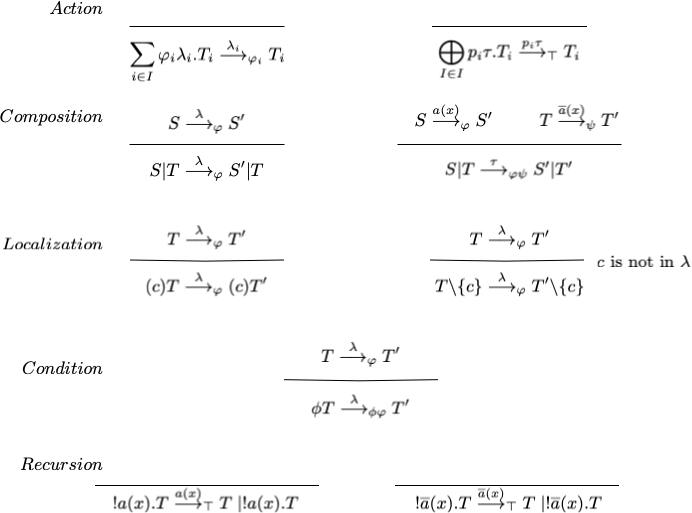
\includegraphics[width=14cm]{../figure/symbolic_sematic.png}
    \caption{\textbf{随机传值进程模型的符号语义}}
    \label{fig_sematic}
\end{figure}

对于$\mathbb{VPC}_{\mathsf{Th}}$的前缀操作子的转移规则:
$\sum_{i\in I} \varphi_i \lambda_i. T_i\stackrel{\lambda_i}{\rightarrow}_{\varphi_i} T_i$,
它本质上代表了非确定选择,
即作出$\varphi_i$条件下的$\lambda_i$动作到达$T_i$状态是非确定的,
我们可以通过Uniform Approach的方法将它扩展为一个概率性选择,
即在概率$p_i$下会作出$\varphi_i$条件下的$\lambda_i$动作:
$\bigoplus_{i\in I} p_i\tau.\varphi_i \lambda_i. T_i\stackrel{p_i\tau}{\rightarrow}_{\top}\stackrel{\lambda_i}{\rightarrow}_{\varphi_i} T_i$。
它的语义为:在概率$p_i$下,我们会经过一个内部$\tau$操作到达一个$\mathbb{RVPC}_{\mathsf{Th}}$状态:
$\varphi_i\lambda_i.T_i$,
若$\mathsf{Th}\vdash \varphi_i$(即一阶理论$\mathsf{Th}$下,$\varphi_i$为真),
则我们可以经过$\lambda_i$操作到达$\mathbb{RVPC}_{\mathsf{Th}}$状态$T_i$, 
其中$\lambda_i \in \{a(x),\bar{a}(x)\mid a\in \mathcal{N}, x\in \mathsf{V}_\Sigma, t\in \mathsf{T}_\Sigma\}\cup \{\tau\}$。

$\mathbb{RVPC}_{\mathsf{Th}}$在$\mathbb{VPC}_{\mathsf{Th}}$的基础上扩展了前缀操作:$p\tau.$,
其中$p\in (0,1)$。
类似$A=\tau.B$的$\mathbb{RVPC}_{\mathsf{Th}}$项,
我们可以认为$A\stackrel{1\tau}{\rightarrow}_{\top} B$,
这时也满足$A=\bigoplus_{i\in I} p_i\tau.A_i$的定义,
此时$I=[1],p_1=1,A_1=B$。
若将$\mathbb{VPC}_{\mathsf{Th}}$中的此类内部操作同样看待,
我们可以得出推论~\ref{co:vpc}。
\begin{corollary}\label{co:vpc}
   $\mathbb{VPC}_{\mathsf{Th}}$是一种特殊的$\mathbb{RVPC}_{\mathsf{Th}}$。
\end{corollary}

\section{随机传值进程模型中的互模拟关系}

\subsection{互模拟关系与观察等价性}\label{ch:bisimulation}

   程序理论的基本问题是进程的等价性。对通信并发系统程序等价的定义和验证,现在已有很多研究。
   在提出CCS时Milner提出了\textit{观察等价(observation equivalence)},即\textit{弱互模拟(weak bisimulation)}\cite{2}。
   Glabbeek和Weijland提出的\textit{分支互模拟(branching bisimulation)}\cite{6}也是十分著名的研究。

   对于概率模型的等价性,目前有对同步概率进程模型互模拟关系的研究\cite{13},
   仅适用于有限状态的概率进程模型的研究\cite{14,15}。
   Uniform Approach在分支互模拟\cite{6}的基础上给出了
   RCCS分支互模拟关系的定义,以及等价关系同余性的证明。
   \subsubsection{Uniform Approach中的分支互模拟}
   分支互模拟涉及等价集的概念,我们首先看CCS等价集的定义:
   \begin{definition}
      若二元关系$\mathcal{E}$是$\mathcal{P}_{CCS}$上的等价关系。
      $A$关于等价关系$\mathcal{E}$的等价集写作$[A]_{\mathcal{E}}$,
      $A\in [A]_{\mathcal{E}}$且$\forall B,(A,B)\in \mathcal{E}$,
      有$B\in [A]_{\mathcal{E}}$。
      我们用$\mathcal{P}_{CCS}/\mathcal{E}$表示所有$\mathcal{P}_{CCS}$关于$\mathcal{E}$的等价集的集合。
   \end{definition}
   $\mathcal{P}_{RCCS}$,$\mathcal{T}_{\mathbb{VPC}_{\mathsf{Th}}}$,$\mathcal{T}_{\mathbb{RVPC}_{\mathsf{Th}}}$上的等价集的定义都是相似的,因此不做赘述。

   RCCS的分支互模拟是CCS分支互模拟的扩展,我们首先来看CCS的分支互模拟。
   $\mathcal{P}_{CCS}$上的分支互模拟的定义如下,其中内部操作$\tau$带来的状态迁移可以称为\textit{静态转移},
   当$A\stackrel{\tau}{\rightarrow}A'\mathcal{E}A$时,我们可以写为$A\stackrel{\tau}{\rightarrow}_{\mathcal{E}}A'$,在Uniform Approach中,这种动作称为\textit{状态保持的静态转移(state-preserving silent transition)},
   对应的若$A\stackrel{\tau}{\rightarrow}A'\notin [A]_{\mathcal{E}}$,称为\textit{状态改变的静态转移}。
   $\Rightarrow_{\mathcal{E}}$为$\stackrel{\tau}{\rightarrow}_{\mathcal{E}}$的闭包。
   \begin{definition}
      $\mathcal{E}$是$\mathcal{P}_{CCS}$上的等价关系,
      若对于任意动作$l,l\neq \tau$和任意等价集$\mathcal{C}\in \mathcal{P}_{CCS}/\mathcal{E}, \mathcal{C}\neq [A]_{\mathcal{E}}$,
      满足若$B\mathcal{E}A\Rightarrow_{\mathcal{E}}\stackrel{l}{\rightarrow}\mathcal{C}$,则$B\Rightarrow_{\mathcal{E}}\stackrel{l}{\rightarrow}\mathcal{C}$,
      称$\mathcal{E}$是$\mathcal{P}_{CCS}$上的分支互模拟关系。
   \end{definition}

   考虑到RCCS在CCS的基础上增加了概率选择,
   状态保持的静态转移在$A\stackrel{\tau}{\rightarrow}A'\mathcal{E}A$的基础上新增了
   $A\stackrel{p\tau}{\rightarrow} A'\mathcal{E}A,0<p<1$的可能,
   为了用类似$\Rightarrow_{\mathcal{E}}$的方式表示这种静态转移,
   Uniform Approach提出了\textit{等价树(Epsilon Tree)}的概念[cite],
   将概率选择作为树的分支,节点$A$的关于等价关系$\mathcal{E}$的等价树上的任意节点$N\in [A]_{\mathcal{E}}$。
   同时,Uniform Approach定义了两种转移:$l$-transition和$q$-transition,
   分别表示等价树上的节点迁移到其他等价集动作和概率。

   \begin{definition}[$l$-转移($l$-transition)]
      $A\in \mathcal{P}_{RCCS}$,
      从$A$到$\mathcal{B}\in \mathcal{P}_{RCCS}/\mathcal{E},\mathcal{B}\neq [A]_{\mathcal{E}}$的
      $l$-转移表示$A$关于等价关系$\mathcal{E}$的等价树上的每一个叶子结点$L$,
      存在$L\stackrel{l}{\rightarrow}L'\in\mathcal{B},l\neq \tau$,写作$A\rightsquigarrow_{\mathcal{E}}\stackrel{l}{\rightarrow}\mathcal{B}$。
   \end{definition}

   \begin{definition}[$q$-转移($q$-transition)]
      $A\in \mathcal{P}_{RCCS}$,$\mathcal{E}$为$\mathcal{P}_{RCCS}$上的等价关系,
      $L$为$A$关于等价关系$\mathcal{E}$的等价树上的每一个叶子结点,
      $\mathcal{B}\in \mathcal{P}_{RCCS}/\mathcal{E}, \mathcal{B}\neq [A]_{\mathcal{E}}$。

      定义$\mathsf{P}(L\stackrel{\coprod_{i\in[k]}p_i\tau}{\longrightarrow}\mathcal{B})=\sum \{p_i|L\stackrel{p_i\tau}{\longrightarrow}L_i\in \mathcal{B}\wedge i\in I\}$。
      
      定义$\mathsf{P}_{\mathcal{E}}(L\stackrel{\coprod_{i\in[k]}p_i\tau}{\longrightarrow}\mathcal{B})=\mathsf{P}(L\stackrel{\coprod_{i\in[k]}p_i\tau}{\longrightarrow}\mathcal{B})/(1-\mathsf{P}(L\stackrel{\coprod_{i\in[k]}p_i\tau}{\longrightarrow}[A]_{\mathcal{E}}))$。

      当$\mathsf{P}_{\mathcal{E}}(L\stackrel{\coprod_{i\in[k]}p_i\tau}{\longrightarrow}\mathcal{B})=q$时,
      记为$A\rightsquigarrow_{\mathcal{E}}\stackrel{q}{\rightarrow}\mathcal{B}$,即$q$-转移。
   \end{definition}

   现在我们终于可以引入Uniform Approach中定义的RCCS的分支互模拟关系了!

   \begin{definition}
      当$\mathcal{P}_{RCCS}$上的等价关系$\mathcal{E}$满足:
      \begin{itemize}
         \item {
            若$B\mathcal{E}A\rightsquigarrow_{\mathcal{E}}\stackrel{l}{\rightarrow}\mathcal{C}\in \mathcal{P}_{RCCS}/\mathcal{E}, l\neq \tau \wedge \mathcal{C}\neq [A]_{\mathcal{E}}$,则$B\rightsquigarrow_{\mathcal{E}}\stackrel{l}{\rightarrow}\mathcal{C}$。
         }
         \item {
            若$B\mathcal{E}A\rightsquigarrow_{\mathcal{E}}\stackrel{q}{\rightarrow}\mathcal{C}\in \mathcal{P}_{RCCS}/\mathcal{E}, l\neq \tau \wedge \mathcal{C}\neq [A]_{\mathcal{E}}$,则$B\rightsquigarrow_{\mathcal{E}}\stackrel{q}{\rightarrow}\mathcal{C}$。
         }
      \end{itemize}
      则等价关系$\mathcal{E}$是分支互模拟关系。
   \end{definition}
   \subsubsection{$\mathbb{VPC}_\mathsf{Th}$的符号互模拟}
   $\mathbb{VPC}_{\mathsf{Th}}$与CCS的区别主要体现在前缀操作子和条件操作子。
   对于前缀操作子,相似的定义互模拟关系是比较容易的,只需要保证通道一致,值一致即可。
   而条件操作子给互模拟的定义带来了麻烦,比如:
   $A=\overline{a}(0).S$和$B=((x=0) \overline{a}(0).S|\urcorner (x=0) \overline{a}(0).S)$在观察上应该是一致的,
   这就要求$B$的两个操作:$B\stackrel{\overline{a}(0)}{\longrightarrow}_{x=0} S$和$B\stackrel{\overline{a}(0)}{\longrightarrow}_{\urcorner (x=0)} S$共同模拟$A\stackrel{\overline{a}(0)}{\longrightarrow}_{\top} S$。
   为解决这一问题,The Value-Passing Calculus提出了符号互模拟:
   \begin{definition}[符号互模拟]\label{def:symbolic_bisimulation}
      $\mathcal{E}$是一个$\mathcal{T}_{\mathbb{VPC}_{\mathsf{Th}}}$上的二元对称关系,
      当$A\mathcal{E}B$满足下列条件时,称$\mathcal{E}$是一个符号互模拟关系:
      \begin{itemize}
         \item {
            若$A\stackrel{\tau}{\rightarrow}_{\varphi} A'$,则存在$\varphi$的划分$\{\varphi_i\}_{i\in I}$和集合$\{B\Rightarrow_{\psi_i} B_i\}_{i\in I}$,
            对于$\forall i\in I$,$\mathsf{Th}\vdash \varphi_i\Rightarrow \psi_i\wedge \varphi_i A\mathcal{E} \varphi_i B_i$,
            且满足$\varphi_i A'\mathcal{E} \varphi_i B_i$或$B_i\stackrel{\tau}{\rightarrow}_{\psi_i'}B_i'\wedge \mathsf{Th}\vdash \varphi_i\Rightarrow \psi_i'\wedge \varphi_i A'\mathcal{E} B_i'$。
         }
         \item {
            若$A\stackrel{\overline{a}(t)}{\rightarrow}_{\varphi} A'$,则存在$\varphi$的划分$\{\varphi_i\}_{i\in I}$和集合$\{B\Rightarrow_{\psi_i}B_i\stackrel{\overline{a}(t_i)}{\rightarrow}_{\psi_i'}B_i'\}$,
            满足$\mathsf{Th}\vdash (\varphi_i\Rightarrow \psi_i\psi_i')\wedge (\varphi_i \Rightarrow t=t_i)$且$(\varphi_i A\mathcal{E}\varphi_i B_i)\wedge(\varphi_i A'\mathcal{E}\varphi_i B_i')$。
         }
         \item {
            若$A\stackrel{a(x)}{\rightarrow}_{\varphi} A'$,则存在$\varphi$的划分$\{\varphi_i\}_{i\in I}$和集合$\{B\Rightarrow_{\psi_i}B_i\stackrel{a(x)}{\rightarrow}_{\psi_i'}B_i'\}$,
            满足$\mathsf{Th}\vdash \varphi_i\Rightarrow \psi_i\psi_i'$且$(\varphi_i A\mathcal{E}\varphi_i B_i)\wedge(\varphi_i A'\mathcal{E}\varphi_i B_i')$。
         }
      \end{itemize}
      最大的互模拟关系记为$\approxeq_{\mathsf{Th}}^s$。
   \end{definition}

   根据符号互模拟的定义,我们可以解决前述条件操作子带来的麻烦,
   我们可以通过下面的例子证明这一点。
   \begin{example}
      证明$A=\overline{a}(0).S$和$B=((x=0) \overline{a}(0).S|\urcorner (x=0) \overline{a}(0).S)$是符号互模拟的。
   \end{example}
   \begin{proof}
      定义等价关系$\mathcal{E}=\{(A,B)\}\cup \equiv$,
      其中$\equiv$为绝对等价关系,
      题目等价于证明$\mathcal{E}$是一个符号互模拟关系。

      对于$A\stackrel{\overline{a}(0)}{\rightarrow}_{\top} S$,
      存在$\top$的划分$\{(x=0),\urcorner(x=0)\}$和集合
      $\{B\stackrel{\overline{a}(0)}{\longrightarrow}_{x=0}S, B\stackrel{\overline{a}(0)}{\longrightarrow}_{\urcorner(x=0)}S\}$,
      且$(x=0)S\mathcal{E}(x=0)S$。

      对于$B\stackrel{\overline{a}(0)}{\longrightarrow}_{x=0}S$,存在$A\stackrel{\overline{a}(0)}{\longrightarrow}_{x=0}S$与之符号互模拟。
      $B\stackrel{\overline{a}(0)}{\longrightarrow}_{\urcorner(x=0)}S$同理。
   \end{proof}

   \subsection{条件等价集}

   根据~\ref{ch:bisimulation}中定义~\ref{def:symbolic_bisimulation}中定义的$\mathbb{VPC}_{\mathsf{Th}}$的符号互模拟关系,
   我们观察$A(x)=(x\geq 5)\overline{a}(\mathsf{s}(x)).0)$和$A'(x)=(x\geq 3)\overline{a}(\mathsf{s}(x)).0$,
   根据$\mathbb{VPC}_\mathsf{Th}$的符号互模拟的定义,我们容易得到$A$和$A'$是不符号互模拟的,
   对于$A'(t)\stackrel{\overline{a}(\mathsf{s}(t))}{\longrightarrow}_{x\geq 3} 0$,
   因为$3<x<5$的这一部分动作是$A(x)$无法完成的,所以不存在$x\geq 3$的划分,
   使得$A(x)$可以给出一个转移的集合来模拟整个$x\geq 3$。
   但反观$B(x)=(x>5)A(x),B'(x)=(x>5)A'(x)$,
   我们可以得到$B'(x)=((x>5)\wedge(x\geq 3))\overline{a}(\mathsf{s}(x)).0=(x>5)\overline{a}(\mathsf{s}(x)).0$,
   同理$B(x)=(x>5)\overline{a}(\mathsf{s}(x)).0$,
   $B(x),B'(x)$不仅是符号互模拟,甚至是绝对等价的。
   对于$(x>5)A(x)$和$(x>5)A'(x)$的这种关系,
   我们给出\textit{条件等价集}的定义,可以使等价集内部对某个条件透明:

   \begin{definition}[条件等价集]
     $A,A'\in \mathcal{T}_{\mathbb{RVPC}_{\mathsf{Th}}}$,$\mathcal{E}$是$\mathbb{RVPC}_{\mathsf{Th}}$上的等价关系,
     若$\varphi A \mathcal{E} \varphi A'$,则$A'\in [A]_{\varphi \mathcal{E}}$。
     $[A]_{\varphi \mathcal{E}}$称为等价关系$\mathcal{E}$在条件$\varphi$下包含$A$的等价集。 
     我们用$\mathcal{T}_{\mathbb{RVPC}_{\mathsf{Th}}}/\varphi \mathcal{E}$表示所有$\mathbb{RVPC}_{\mathsf{Th}}$关于布尔表达式$\varphi$和等价关系$\mathcal{E}$的条件等价集的集合。 
   \end{definition} 

   由于$\mathbb{VPC}_{\mathsf{Th}}$是特殊的$\mathbb{RVPC}_{\mathsf{Th}}$,
   条件等价集的定义同样适用$\mathbb{VPC}_{\mathsf{Th}}$。
   显然,$A'(x)\in [A(x)]_{(x>5)\mathcal{E}}$,其中$\mathcal{E}=\approxeq_{\mathsf{Th}}^s$。
   
   条件$\top$具有一定的特殊性:
   对于无条件的操作我们认为操作是在$\top$条件下执行的,
   因此$\top$可以看作是最强的条件。

   \begin{corollary}
      $A,B\in \mathcal{T}_{\mathbb{VPC}_{\mathsf{Th}}}$,
      $A\approxeq_{\mathsf{Th}}^sB$,则对于任意布尔表达式$\varphi'$,$\varphi' A\approxeq_{\mathsf{Th}}^s\varphi' B$。
   \end{corollary}
   \begin{proof}
      对于$A$可以执行的操作,$\varphi' A$也会有对应的版本:
      \begin{itemize}
         \item 若$A\stackrel{\tau}{\rightarrow}_{\varphi} A'$,则$\varphi' A\stackrel{\tau}{\rightarrow}_{\varphi' \varphi}A'$。
         \item 若$A\stackrel{a(x)}{\rightarrow}_{\varphi} A'$,则$\varphi' A\stackrel{a(x)}{\rightarrow}_{\varphi' \varphi} A'$。
         \item 若$A\stackrel{\overline{a}(t)}{\rightarrow}_{\varphi} A'$,则$\varphi' A\stackrel{\overline{a}(t)}{\rightarrow}_{\varphi' \varphi} A'$。
      \end{itemize}
      对$\varphi' A\stackrel{a(x)}{\rightarrow}_{\varphi'\varphi} A'$,
      根据$A\approxeq_{\mathsf{Th}}^sB$,我们知道存在$\varphi$的划分$\{\varphi_i\}_{i\in I}$和集合$\{B\Rightarrow_{\psi_i}B_i\stackrel{a(x)}{\rightarrow}_{\psi_i'}B_i'\}_{i\in I}$,
      满足$\mathsf{Th}\vdash \varphi_i\Rightarrow \psi_i \psi_i' \wedge \varphi_i A\approxeq_{\mathsf{Th}}^s \varphi_i B_i \wedge \varphi_i A'\approxeq_{\mathsf{Th}}^s \varphi_i B_i'$。
      
      若要证明$\varphi' A\approxeq_{\mathsf{Th}}^s\varphi' B$,
      我们可以构造等价关系$\mathcal{S} = \{(\varphi'A,\varphi'B)|A,B\in \approxeq_{\mathsf{Th}}^s\}$,
      证明$\mathcal{S}$是符号互模拟的(这样假设的原因是题目中的$A,B$原本也是任意的)。

      通过$A\approxeq_{\mathsf{Th}}^sB$我们可以得到集合$\{\varphi'\varphi_i\}_{i\in I}$,
      对于任意$i,j$,由于$\varphi_i \wedge \varphi_j = \bot$,
      我们可以得到$(\varphi'\varphi_i) \wedge (\varphi'\varphi_j) = \bot$;
      又$\bigvee_{i\in I}\varphi_i = \varphi$,$\bigvee_{i\in I}\varphi'\varphi_i = \varphi'\varphi$,
      因此$\{\varphi'\varphi_i\}_{i\in I}$为$\varphi'\varphi$的划分。
      我们还可以得到集合$\{\varphi'B\Rightarrow_{\varphi'\psi_i}B_i\stackrel{a(x)}{\rightarrow}_{\psi_i'} B_i'\}$,
      满足$\mathsf{Th}\vdash \varphi'\varphi_i\Rightarrow \varphi'\psi_i\psi_i'$,
      而$(\varphi'\varphi_i A, \varphi'\varphi_i B_i),(\varphi'\varphi_i A', \varphi'\varphi_i B_i')\in \mathcal{S}$,
      因此我们可以用$\{\varphi'B\Rightarrow_{\varphi'\psi_i}B_i\stackrel{a(x)}{\rightarrow}_{\psi_i'} B_i'\}$模拟$\varphi' A\stackrel{a(x)}{\rightarrow}_{\varphi'\varphi} A'$。

      对称的一边和其他两种情况的证明是相似的。
   \end{proof}

   \begin{corollary}\label{co:all}
      $A,B\in \mathbb{RVPC}_{\mathsf{Th}}$,$\mathcal{E}$是$\mathbb{RVPC}_{\mathsf{Th}}$上的等价关系,
      $\varphi$是任意布尔表达式,
      若$B\in [A]_{\mathcal{E}}$,则$B\in [A]_{\varphi \mathcal{E}}$。
   \end{corollary}
   
   推论~\ref{co:all}可以简单理解为:一个$\mathbb{RVPC}_{\mathsf{Th}}$项在任意条件下成立的等价集是所有条件等价集的交集。

   将$\top$推广到其他布尔表达式,我们可以得到更为广泛的结论:

   \begin{corollary}
      $A,B\in \mathcal{T}_{\mathbb{VPC}_{\mathsf{Th}}}$,
      若$\varphi A\approxeq_{\mathsf{Th}}^s \varphi B$,
      则对布尔表达式$\varphi',\mathsf{Th}\vdash \varphi\Rightarrow \varphi'$,
      $\varphi' A\approxeq_{\mathsf{Th}}^s\varphi' B$。
   \end{corollary}

   \begin{corollary}\label{co:all_1}
      $A,B\in \mathbb{RVPC}_{\mathsf{Th}}$,$\mathcal{E}$是$\mathbb{RVPC}_{\mathsf{Th}}$上的等价关系,
      $\varphi$是任意布尔表达式,
      若$B\in [A]_{\varphi\mathcal{E}}$,
      则对于布尔表达式$\varphi\Rightarrow \varphi'$,
      $B\in [A]_{\varphi' \mathcal{E}}$。
   \end{corollary}
\subsection{条件等价树}
   定义~\ref{def:symbolic_bisimulation}给出了$\mathbb{VPC}_{\mathsf{Th}}$的互模拟的定义,
   观察定义~\ref{def:symbolic_bisimulation}中的$A\stackrel{a(x)}{\longrightarrow}_{\varphi} A'$,
   我们用$\{B\Rightarrow_{\psi_i}B'_i\stackrel{a(x)}{\longrightarrow}_{\psi'_i}B_i'\}$模拟,
   其中$(\varphi_i A\mathcal{E}\varphi_i B_i)\wedge(\varphi_i A'\mathcal{E}\varphi_i B_i')$,
   根据条件等价集的定义,我们可以得到$B_i\in [A]_{\varphi\mathcal{E}}$,$B_i'\in [A']_{\varphi \mathcal{E}}$,
   由于$B_i \approxeq_{\mathsf{Th}}^s A$,$B_i\approxeq_{\mathsf{Th}}^s B$,那么$B\Rightarrow_{\psi_i}B_i$实际上也是\textit{状态保持的静态转移}。

   对于我们概率扩展后的$\mathbb{RVPC}_{\mathsf{Th}}$,
   对上述例子状态保持静态转移多了$B\stackrel{q\tau}{\rightarrow}_{\psi_i} B_i$
   的情况,其中$q\in(0,1)$,表示\textit{概率的状态保持的静态转移}。
   我们希望可以找到$\mathbb{RVPC}_{\mathsf{Th}}$中类似$\Rightarrow$的方式来表达这种状态保持的静态转移。
   我们可以使用Uniform Approach中等价树的方法来刻画这种状态保持的静态转移,
   在$\mathbb{RVPC}_{\mathsf{Th}}$中称为\textit{条件等价树}。

   在定义条件等价树之前,我们首先关注一种条件无关的静态转移树:
\begin{definition}[静态转移树]
   \label{def:silent_tree}
   若$A\in \mathcal{T}_{\mathbb{RVPC}_{\mathsf{Th}}}$,
   $A$的静态转移树$t$满足如下定义:
   \begin{itemize}
   \item 每一个节点都被标记成$\mathcal{T}_{\mathbb{RVPC}_{\mathsf{Th}}}$的一个项,$A$是根节点。
   \item {
      节点间的边被标记成$(\varphi,p)$,其中$p\in(0,1]$,$\varphi$是一个布尔表达式。
      如果一条从$A'$到$A''$的有向边被标记成$(\varphi,p)$,表示$A'\stackrel{p\tau}{\rightarrow}_{\varphi} A''$。
   }
   \end{itemize}
\end{definition}

静态转移树包含了\textit{状态改变的静态转移}和\textit{状态保持的静态转移},
条件等价树需要对特定条件下的状态改变的静态转移进行剪枝:

\begin{definition}[条件等价树]
   $\varphi$是一个布尔表达式,$\mathcal{E}$是$\mathcal{T}_{\mathbb{RVPC}_{\mathsf{Th}}}$上的等价关系,
   $A\in \mathcal{T}_{\mathbb{RVPC}_{\mathsf{Th}}}$,
   当下列条件成立时,$A$的静态转移树$t$称为是一个关于$\varphi\mathcal{E}$的条件等价树($\varphi \mathcal{E}$-tree) ,记作$t^A_{\varphi \mathcal{E}}$。
\begin{itemize}
   \item $t$上的所有节点$N$,$N\in [A]_{\varphi \mathcal{E}}$。
   \item {
   若$t$的边被标记为$(\psi, q)$,则$\mathsf{Th}\vdash \varphi\Rightarrow \psi$。
   }
   \item {
         若$B.B'$是$t$上的节点,
         $B\stackrel{(\psi,q)}{\rightarrow}B',q\in (0,1)$,
         则存在$B\stackrel{\coprod_{i\in [k]}}{\longrightarrow}_{\psi} \coprod_{i\in [k]} B_i$,
         $B_i,i\in [k]$是$t$上的节点,
         且$B$有且仅有$B_1,\dots, B_k$这$k$个儿子节点。
   }
   \item {
      若$B,B'$是$t$上的节点,
      $B\stackrel{(\psi,1)}{\rightarrow}B'$,
      则$B\stackrel{\tau}{\rightarrow}_{\psi}B'$且$B$有且仅有$B'$一个儿子节点。
   }
\end{itemize}
\end{definition}

条件等价树实质上是\textit{概率的状态保持的静态转移}。

从定义上看条件等价树的定义比较抽象,我们可以看几个简单有趣的例子:
\begin{example}
   $H(x)\stackrel{def}{=}(x\leq 3)(\frac{1}{3}\tau.(x\leq 1)G(x)\oplus\frac{1}{3}\tau.(x\leq 2)G(x)\oplus\frac{1}{3}\tau.(x\leq 3)G(x))$

   $[H(x)]_{\mathcal{E}_1} = [G(x)]_{\mathcal{E}_1}$,$H(x),G(x)\in \mathbb{RVPC}_{\mathsf{Th}}$,其中$\mathsf{Th}=\mathsf{PA}$[cite]。

   $H(x)$的静态转移树如图~\ref{fig_eg0_1},它包含了$H(x)$的静态转移。
   \begin{figure}[!htbp]
      \small
      \centering
      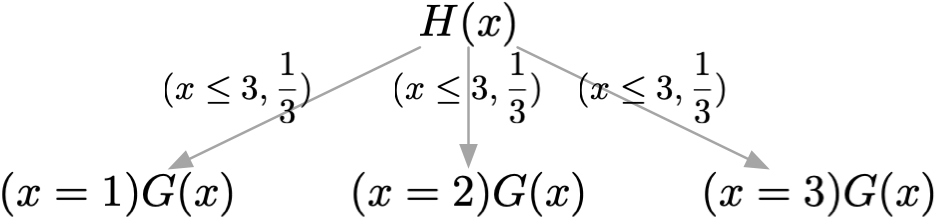
\includegraphics[width=8cm]{../figure/example0_1.png}
      \caption[]{}
      \label{fig_eg0_1}
   \end{figure}

   因为$\mathsf{Th}\vdash \top \not\Rightarrow (x\leq 3)$,
   $H(x)$的$\top\mathcal{E}_1$-tree只有一个根节点$H(x)$。

   同理,$H(x)$的$(x>3)\mathcal{E}_1$-tree只有一个根节点$H(x)$。

   $H(x)$的$(x<2)\mathcal{E}_1$-tree如图~\ref{fig_eg0_2},
   其中$\mathsf{Th}\vdash (x<2)\Rightarrow (x\leq 3)$,
   由于$(x<2)\wedge(x\leq 2)G(x) = (x<2)G(x)$,$G(x)\in[H(x)]_{\mathcal{E}_1}$,
   根据推论~\ref{co:all},$(x\leq 2)G(x)\in [H(x)]_{(x<2)\mathcal{E}_1}$。
   另一个分支同理。
   \begin{figure}[!htbp]
      \small
      \centering
      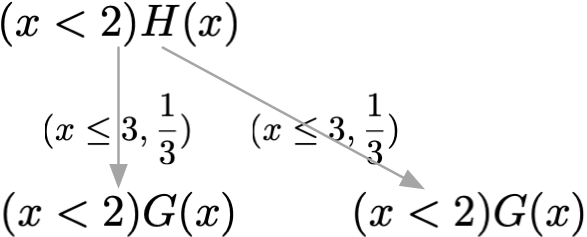
\includegraphics[width=5cm]{../figure/example0_2.png}
      \caption[]{}
       \label{fig_eg0_2}
   \end{figure}
\end{example}
\begin{example}\label{eg:1}
      假设我们有一个不太行的下课铃系统,每一时刻它坏掉的可能性是$\frac{1}{2}$,可以通过内部自动校准系统(静态转移:$\tau$操作)修复,
      它的内部有一个计时器,每隔定长时间($\tau$操作)就会从$a$通道广播录好的一段下课铃,
      录好的下课铃可以用变量$x$表示。
      这个下课铃系统可以被抽象为一个$\mathbb{RVPC}_{\mathsf{Th}}$,其中$\mathsf{Th}$可以认为是$\mathsf{PA}$,
      我们可以用$G(x)$来表示这个系统:
      $$G(x)\stackrel{def}{=}\mu X.(\frac{1}{2}\tau.X\oplus \frac{1}{2}\tau.\overline{a}(x).X)$$
      $G(x)$在$\mathcal{E}_2$的等价集$[G(x)]_{\top\mathcal{E}_2} = [\overline{a}(x).G(x)]_{\top\mathcal{E}_2}$。
      $G(x)$的$\top \mathcal{E}_2$-tree如图~\ref{fig_eg1}。
      \begin{figure}[!htbp]
         \small
         \centering
         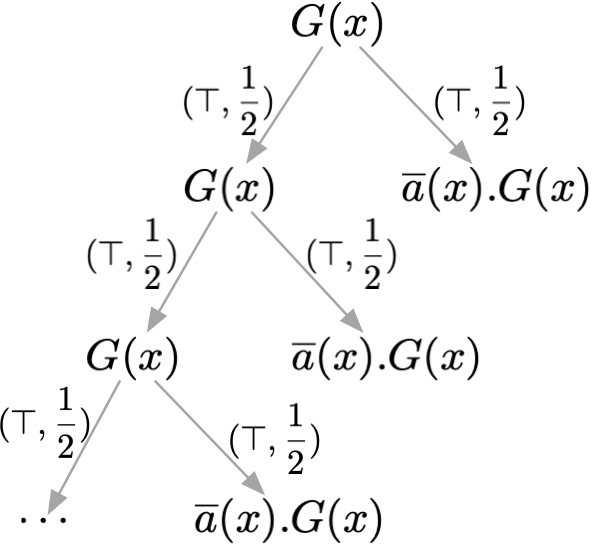
\includegraphics[width=5cm]{../figure/example1.png}
         \caption[]{} 
         \label{fig_eg1}
      \end{figure}
\end{example}
\begin{example}\label{eg:2}
   假设之前的不太行的下课铃系统经过岁月的磨练,年久失修,
   每自动校准一次音量就会减弱,我们用变量$y$来表示音量,
   音量必须满足$y>1$才可以播放,
   当$y\leq 0$时下课铃系统音量就无法减弱了。
   为了方便建模,我们用$\mathsf{p}(x)=x-1$来表示这种音量减弱。
   校长出于节约经费的考虑,只要下课铃还能在他办公室听见($y>3$)就可以继续使用,
   现在的下课铃系统依然是一个$\mathbb{RVPC}_{\mathsf{Th}}$,
   我们可以用修改的$G'(x,y)$来表示这个系统:
   $$G'(x,y)\stackrel{def}{=}(y>3)(\frac{1}{2}\tau.((y>0)\tau.G'(x,\mathsf{p}(y))|\urcorner (y>0)\tau.G'(x,y))\oplus \frac{1}{2}\tau.((y>1)\overline{a}(x).G'(x,y)))$$
   $G'(x,y)$在$(y>3)\mathcal{E}_3$的等价集$[G'(x,y)]_{(y>3)\mathcal{E_3}}=[G'(x,y')]_{(y'>3)\mathcal{E_3}}=[\overline{a}(x).G'(x,y'')]_{(y''>3)\mathcal{E_3}}$,其中$y,y',y''$不一定相等。

   $G'(x,y)$的$(y>3)\mathcal{E}_3$-tree如图~\ref{fig_eg2}。
   \begin{figure}[!htbp]
      \small
      \centering
      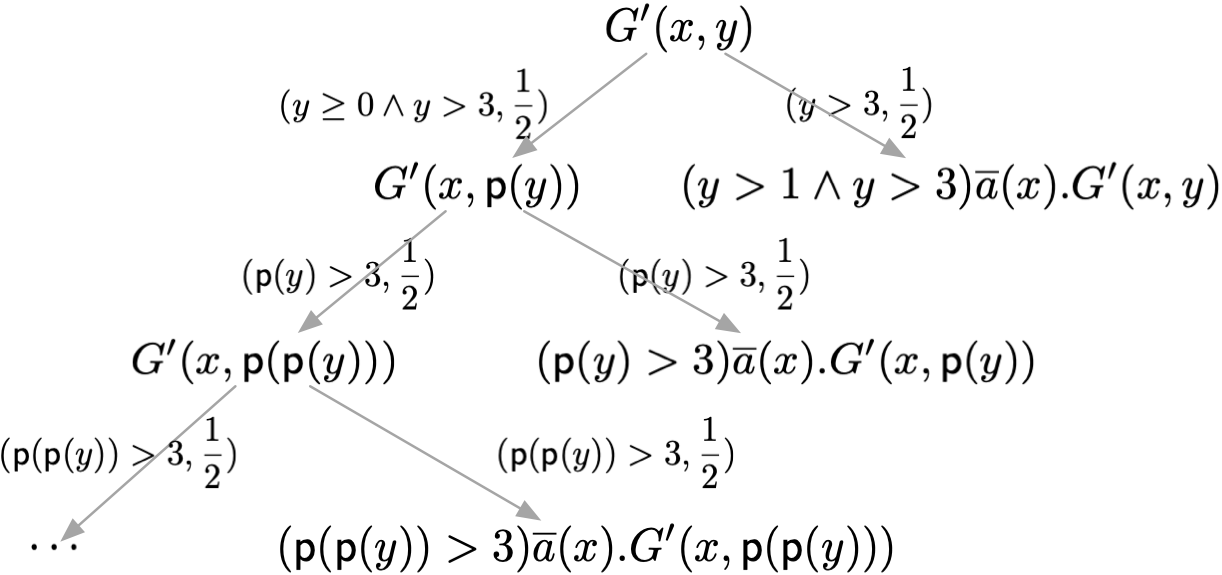
\includegraphics[width=11cm]{../figure/example2.png}
      \caption[]{} 
      \label{fig_eg2}
   \end{figure}

\end{example}

\subsection{随机传值进程模型的符号互模拟}
定义了\textit{概率的状态保持的静态转移},
我们现在可以用Uniform Approach的方法得到$\mathbb{RVPC}_{\mathsf{Th}}$的符号互模拟。
类似的,我们首先需要定义概率版的$l$-转移和$q$-转移。

\begin{definition}[条件$l$-转移($\varphi l$-transition)]
   $A\in \mathcal{T}_{\mathbb{RVPC}_{\mathsf{Th}}}, \mathcal{B}\in \mathcal{T}_{\mathbb{RVPC}_{\mathsf{Th}}}/\varphi'\mathcal{E}\backslash \{[A]_{\varphi'\mathcal{E}}\}$,
   其中$\varphi'$是一个布尔表达式,$\mathcal{E}$是$\mathcal{T}_{\mathbb{RVPC}_{\mathsf{Th}}}$上的等价关系,
   若$A$的条件等价树$t_{\varphi' \mathcal{E}}^A$的所有叶子结点$L$,
   存在$L\stackrel{l}{\rightarrow}_{\varphi} L'\in \mathcal{B},l\neq \tau$,
   称为$A$到$\mathcal{B}$的$\varphi l$-转移,记作$A\rightsquigarrow_{\varphi'\mathcal{E}}\stackrel{l}{\rightarrow}_{\varphi}\mathcal{B}$。
\end{definition}

\begin{definition}[条件$q$-转移($\varphi q$-transition)]
   $A\in \mathcal{T}_{\mathbb{RVPC}_{\mathsf{Th}}},\mathcal{B}\in (\mathcal{T}_{\mathbb{RVPC}_{\mathsf{Th}}}/\varphi' \mathcal{E})\backslash \{[A]_{\varphi'\mathcal{E}}\}$,
   其中$\varphi'$是一个布尔表达式,$\mathcal{E}$是$\mathcal{T}_{\mathbb{RVPC}_{\mathsf{Th}}}$上的等价关系,
   对$t^A_{\varphi' \mathcal{E}}$的每一个叶子结点$L$和布尔表达式$\varphi$,
   若$L\stackrel{\coprod_{i\in I}p_i\tau}{\longrightarrow}_{\coprod_{i\in I}\psi_i} \coprod_{i\in [k]}L_i$,
$i\in I, L_i\in \mathcal{B}$,且$\mathsf{Th}\vdash \varphi \Rightarrow \psi_i$:

定义$\mathsf{P}_\varphi(L\stackrel{\coprod_{i\in I}p_i\tau}{\longrightarrow}_{\coprod_{i\in I}\psi_i}\mathcal{B}) = \sum\{p_i\mid L\stackrel{p_i\tau}{\rightarrow}_{\psi_i} L_i\in\mathcal{B} \wedge i\in I \wedge \mathsf{Th}\vdash \varphi \Rightarrow \psi_i\}$。

定义$\mathsf{P}_{\varphi, \varphi' \mathcal{E}}(L\stackrel{\coprod_{i\in I}p_i\tau}{\longrightarrow}_{\coprod_{i\in I}\psi_i}\mathcal{B}) = \mathsf{P}_\varphi(L\stackrel{\coprod_{i\in I}p_i\tau}{\longrightarrow}_{\coprod_{i\in I}\psi_i}\mathcal{B})/(1-\mathsf{P}_\varphi(L\stackrel{\coprod_{i\in I}p_i\tau}{\longrightarrow}_{\coprod_{i\in I}\psi_i}[A]_{\varphi\mathcal{E}}))$。

当$\mathsf{P}_{\varphi,\varphi' \mathcal{E}}(L\stackrel{\coprod_{i\in I}p_i\tau}{\longrightarrow}_{\coprod_{i\in I}\psi_i}\mathcal{B})=q$时,
称$A$到$\mathcal{B}$存在$\varphi q$-转移。写作$A\rightsquigarrow_{\varphi'\mathcal{E}} \stackrel{q}{\rightarrow}_{\varphi} \mathcal{B}$。
\end{definition}

符号互模拟实质上是保证$\mathcal{T}_{\mathbb{RVPC}_{\mathsf{Th}}}$上的等价关系满足条件$l$-转移和条件$q$-转移。
\begin{definition}[符号互模拟]
   $\mathcal{E}$是一个$\mathcal{T}_{RVPC}$上的二元对称关系,
当$A\mathcal{E}B$且满足下列条件时,称$\mathcal{E}$是一个符号互模拟(Symbolic Bisimulation):
\begin{itemize}
   \item {
      若$ A \rightsquigarrow_{\varphi \mathcal{E}}\stackrel{a(x)}{\rightarrow}_{\varphi} \mathcal{C}\in \mathcal{T}/\varphi\mathcal{E}, \mathcal{C}\neq [A]_{\varphi \mathcal{E}}$,
      则存在$\varphi$的划分$\{\varphi_i\}_{i\in I}$,和集合$\{B\rightsquigarrow_{\psi_i \mathcal{E}}\stackrel{a(x)}{\rightarrow}_{\psi_i'} \mathcal{C}\}$,
      使得对$i\in I$,$\mathsf{Th}\vdash \varphi_i \Rightarrow \psi_i\psi_i'$。
   }
   \item {
      若$A \rightsquigarrow_{\varphi \mathcal{E}}\stackrel{\bar{a}(t)}{\rightarrow}_{\varphi} \mathcal{C}\in \mathcal{T}/\varphi\mathcal{E},\mathcal{C}\neq [A]_{\varphi\mathcal{E}}$,
      则存在$\varphi$的划分$\{\varphi_i\}_{i\in I}$,和集合$\{B\rightsquigarrow_{\psi_i\mathcal{E}}\stackrel{\bar{a}(t_i)}{\rightarrow}_{\psi_i'} \mathcal{C}\}$,
      使得对$i\in I$,$\mathsf{Th}\vdash (\varphi_i \Rightarrow \psi_i\psi_i')\wedge \varphi_i \Rightarrow (t=t_i)$。
   }
   \item {
      若$ A\rightsquigarrow_{\varphi\mathcal{E}} \stackrel{q}{\rightarrow}_{\varphi} \mathcal{C}\in \mathcal{T}/\mathcal{E}, \mathcal{C}\neq [A]_{\varphi \mathcal{E}}$,
      则$B\rightsquigarrow_{\varphi \mathcal{E}} \stackrel{q}{\rightarrow}_{\varphi} \mathcal{C}$
   }
\end{itemize}
\end{definition}

在证明$\mathcal{T}_{\mathbb{RVPC}_{\mathsf{Th}}}$的两项符号互模拟时,
我们通常可以构造一个含有该项的等价集,并证明该等价集是一个符号互模拟关系。
构建一个$\mathcal{T}_{\mathbb{RVPC}_{\mathsf{Th}}}$项的条件$l$-转移和条件$q$-转移时,
我们可以首先构建该项的\textit{静态转移树}。

\begin{example}
   假设学校负责看管设备的老师发现例~\ref{eg:2}中的下课铃系统其实只有在$y\geq 5$时才能被所有教室的同学们听到,
   为了不违抗校长的决定又同时让同学们都听到下课铃,他决定当$(y<5)$时用自己的电脑通过$a$通道播放下课铃,
   这时校长以为下课铃系统被工人修好成~\ref{eg:1}中的样子了,决定一直使用这个下课铃。校长的感觉是错觉吗?

   此时,看管设备的老师和之前不太行的下课铃系统依旧是一个Random VPC,我们可以用$G''(x,y)$来表示:

   $G''(x,y) = (\frac{1}{2}\tau.((y>0)\tau.G''(x,\mathsf{p}(y))|\urcorner (y>0)\tau.G''(x,y))\oplus \frac{1}{2}\tau.((y>1)\overline{a}(x).G''(x,y)|(y<5)\overline{a}(x).G''(x,y))$。

   我们只需要证明$G(x)$与$G''(x,y)$符号互模拟即可。
\end{example}
\begin{proof}
   设等价集$\mathcal{S} = \{(G(t),G''(t,s)),(G(t),(y>0)\tau.G''(x,\mathsf{p}(y))|\urcorner (y>0)\tau.G''(x,y)),(\overline{a}.G(t),(s>1)\overline{a}(t).G''(t,s)|(s<5)\overline{a}(t).G''(t,s))\mid t\in V,s\in U\}$,$V$是$x$的所有赋值的集合,$U$是$y$的所有赋值的集合,
   我们只需证明$\mathcal{S}$是一个符号互模拟关系即可。
   \begin{itemize}
      \item {
         $\overline{a}(x).G(x)$和$(y>1)\overline{a}(x).G''(x,y)|(y<5)\overline{a}(x).G''(x,y)$的$\top\mathcal{S}$-tree只有一个根节点(这里的证明实际可以是$\mathbb{VPC}$的符号互模拟的证明,但可以使用Random VPC的证明方式,下面用Random VPC的证明),
         \begin{itemize}
            \item {
               对于$x$的每一个赋值$t$,
               $\overline{a}(x).G(x)\rightsquigarrow_{\top\mathcal{S}}\stackrel{\overline{a}(t)}{\longrightarrow}_{\top}G(t)$。
               我们可以得到$\top$的一个划分:$\top=(y>1)\vee (y\leq 1)$。
      
               这时存在集合
               $$\{(y>1)\overline{a}(x).G''(x,y)|(y<5)\overline{a}(x).G''(x,y)\rightsquigarrow_{(y>1)\mathcal{S}}\stackrel{\overline{a}(t)}{\rightarrow}_{(y>1)}G''(t,s),$$
               $$(y>1)\overline{a}(x).G''(x,y)|(y<5)\overline{a}(x).G''(x,y)\rightsquigarrow_{(y\leq 1)\mathcal{S}}\stackrel{\overline{a}(t)}{\rightarrow}_{(y<5)}G''(t,s)\}$$
               可以模拟上述操作。
            }
            \item {
               对$x$的每一个赋值$t$,
               $(y>1)\overline{a}(x).G''(x,y)|(y<5)\overline{a}(x).G''(x,y)\rightsquigarrow_{(y>1)\mathcal{S}}\stackrel{\overline{a}(t)}{\rightarrow}_{(y>1)}G''(t,s)$,
               存在集合$\{\overline{a}(x).G(x)\rightsquigarrow_{(y>1)\mathcal{S}}\stackrel{\overline{a}(t)}{\longrightarrow}_{(y>1)}G(t)\}$可以模拟上述操作。
               另一个操作的证明是相似的。
            }
         \end{itemize}
      }
      \item {
         $(G(t),(y>0)\tau.G''(x,\mathsf{p}(y))|\urcorner (y>0)\tau.G''(x,y))$的这一对等价关系也是常规的$\mathcal{VPC}$证明[此处应有引用]。
      }
      \item {
         $G(x)$的静态转移树如图~\ref{fig_eg4_1},$G''(x,y)$的静态转移树如图~\ref{fig_eg4_2}。
         \begin{figure}[!htbp]
            \caption[]{}
            \small
            \centering
            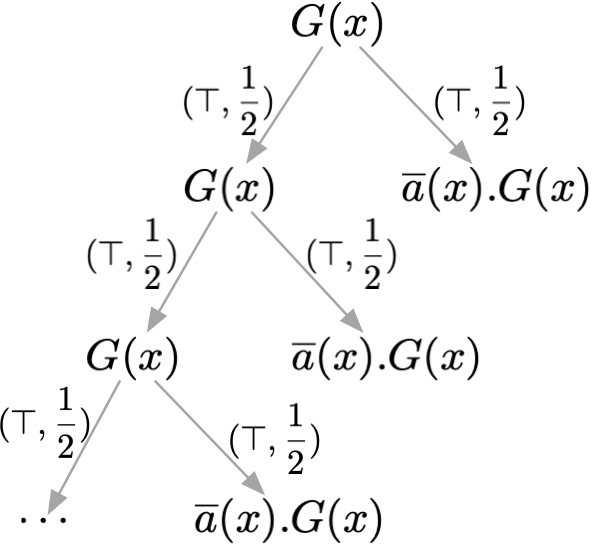
\includegraphics[width=5cm]{../figure/example1.png}
             \label{fig_eg4_1}
         \end{figure}
         \begin{figure}[!htbp]
            \caption[]{}
            \small
            \centering
            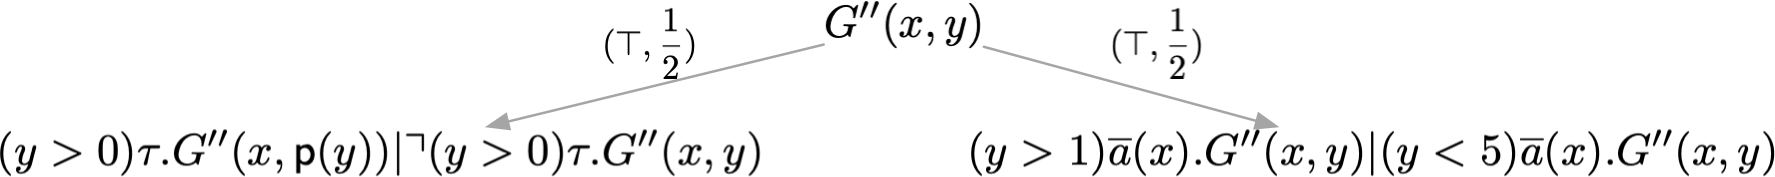
\includegraphics[width=13cm]{../figure/example4_2.png}
             \label{fig_eg4_2}
         \end{figure}

         对于$G(x)\rightsquigarrow_{\top\mathcal{S}}\stackrel{\frac{1}{2}}{\rightarrow}_{\top} [\overline{a}(x).G(x)]_{\top\mathcal{S}}$,
         我们可以用$G''(x,y)\rightsquigarrow_{\top\mathcal{S}}\stackrel{\frac{1}{2}}{\rightarrow}_{\top}[(y>1)\overline{a}(x).G''(x,y)|(y<5)\overline{a}(x).G''(x,y)]_{\top\mathcal{S}}$模拟。
         对称的,因为$\mathcal{S}$是一个等价关系,具有传递性,$(G(x),G''(x,y))\in\mathcal{S}\wedge (G(x),(y>0)\tau.G''(x,\mathsf{p}(y))|\urcorner (y>0)\tau.G''(x,y))\Rightarrow (y>0)\tau.G''(x,\mathsf{p}(y))|\urcorner (y>0)\tau.G''(x,y)\in [G(x)]_{\top\mathcal{S}}$,
         我们也只需要证明右侧的转移,右侧的转移是相似的。
      }
   \end{itemize}
   因此我们可以得出校长的判断是正确的。
\end{proof}

\begin{theorem}
   若$S,T\in \mathcal{T}_{RVPC},S\approxeq^s_{\mathsf{Th}} T$,则$\varphi S \approxeq^s_{\mathsf{Th}} \varphi T$,$\varphi$是一个判定条件。
\end{theorem}
该定理的证明在下一节。

\section{随机传值进程模型的等价性}

\begin{lemma}
   符号互模拟具有传递性。
\end{lemma} 
\begin{proof}
   即证明若$\mathcal{E}$是一个symbolic bisimulation,$A\mathcal{E}B, B \mathcal{E} C$,则$A \mathcal{E} C$。
   \begin{itemize}
      \item {
         若$A\rightsquigarrow_{\varphi \mathcal{E}}\stackrel{\lambda}{\rightarrow} \mathcal{C}\in \mathcal{T}_{RVPC}/\varphi\mathcal{E}$,
         由于$A\mathcal{E}B$根据定义存在$\varphi$的划分$\{\varphi_i\}$和集合$\{B\rightsquigarrow_{\varphi_i\mathcal{E}}\stackrel{\lambda}{\rightarrow}_{\psi}\mathcal{C}|\mathsf{Th}\vdash \varphi_i\Rightarrow\psi_i\}$。
         对于每一个$B\rightsquigarrow_{\varphi_i\mathcal{E}}\stackrel{\lambda}{\rightarrow}_{\psi_i}\mathcal{C}$,
         $t^B_{\varphi_i\mathcal{E}}$上的每一个结点一定属于$[B]_{\psi_i\mathcal{E}}$,
         所以$t^b_{\varphi_i\mathcal{E}}$实际上是$t^b_{\psi_i\mathcal{E}}$的子树,
         $B\rightsquigarrow_{\varphi_i\mathcal{E}}\stackrel{\lambda}{\rightarrow}_{\psi_i}\mathcal{C}$中的起点终点对$\{(M,N)|(M\in t^B_{\varphi_i\mathcal{E}})\vee(N\in \mathcal{C}) \vee (M\stackrel{\lambda}{\rightarrow}_{\psi_i}N))\}$是
         $B\rightsquigarrow_{\psi_i\mathcal{E}}\stackrel{\lambda}{\rightarrow}_{\psi_i}\mathcal{C}$中的起点终点对$\{(M',N')|(M'\in t^B_{\psi_i\mathcal{E}})\vee(N'\in \mathcal{C}) \vee (M'\stackrel{\lambda}{\rightarrow}_{\psi_i}N'))\}$的子集。
         由于$B\mathcal{E}C$,对于每一个$B\rightsquigarrow_{\psi_i}\stackrel{\lambda}{\rightarrow}_{\psi_i}\mathcal{C}$,
         根据定义存在$\psi_i$的划分$\{\psi_{i,j}\}$和集合$S=\{C\rightsquigarrow_{\psi_{i,j}\mathcal{E}}\stackrel{\lambda}{\rightarrow}_{\phi_{i,j}}\mathcal{C}|\mathsf{Th}\vdash \psi_{i,j}\Rightarrow \phi_{i,j}\}$,
         那么存在$S$的子集$S'$的可以模拟$B\rightsquigarrow_{\varphi_i\mathcal{E}}\stackrel{\lambda}{\rightarrow}_{\psi_i}\mathcal{C}$。
   
         我们只需要再构建$\varphi$的划分$\{\varphi_i'\}_{i\in I}$使其一一对应$S'$中涉及的条件$\{\phi_{i,k}\}_{k\in K}\subset\{\phi_{i,j}\}_{j\in J}$即可。
         由于存在$\psi_i$的划分$\{\psi_{i,j}\}_{j\in J}$满足$\psi_{i,j}\Rightarrow \phi_{i,j}\}_{j\in J}$,
         那么我们可以构造$Con=\{\psi_{i,k}\}_{k\in [K-1]}\cup\{\bigvee_{j\in J/[K-1]}\psi_{i,j}\}$,
         对$c_k\in Con, \bigvee_{k\in K}c_k \Leftrightarrow \psi_i$, 且$Con$中元素两两互斥。
         我们用$(\bigvee Con_i)\wedge \varphi_i$代替$\varphi_i$,即可得到最终的划分。
      }
      \item {
         $\varphi q$-transition的传递性与以上过程相似。
      }
   \end{itemize}
\end{proof}
\begin{lemma}
   如果每一个$\mathcal{T}_{RVPC}$上的关系$\mathcal{E}_i$都是符号互模拟,那么$(\bigcup_{i\in I}\mathcal{E}_i)^*$是符号互模拟。
\end{lemma}
\begin{proof}
   令$\mathcal{E}=(\bigcup_{i\in I}\mathcal{E}_i)^*$。若因为$\varphi A_0\mathcal{E}_1 \varphi A_1 \mathcal{E}_2 \dots \mathcal{E}_k \varphi A_k$ ,
$(\varphi A_0, \varphi A_k)\in \mathcal{E}$,由于互模拟具有传递性,通过依次证明$A_0\mathcal{E}A_1, A_1\mathcal{E}A_2 \dots$,我们可以证明$A_0$和$A_k$互模拟。

我们可以通过$A_0$的$\varphi\mathcal{E}$-tree,$t_{A_0}$递归的构建$A_1$的$\varphi\mathcal{E}$-tree,$t_{A_1}$,
进而对$A_0\rightsquigarrow_{\varphi\mathcal{E}}\stackrel{\lambda}{\rightarrow}_{\varphi}\mathcal{C}$构造出$\{A_1\rightsquigarrow_{\varphi_i\mathcal{E}}\stackrel{\lambda}{\rightarrow}_{\psi_i} \mathcal{C}|\mathsf{Th}\vdash (\varphi_i\Rightarrow\psi_i)\vee (\textrm{$\{\varphi_i\}$是$\varphi$的一个划分})\}$。
对于每次递归的$t_{A_0}$的根结点,分以下情况讨论:

\begin{itemize}
   \item {
      \textbf{Case 1 $t_{A_0}$的根结点只有一个儿子$A_0'$。}
      \begin{itemize}
         \item {
            \textbf{Case 1.1 $A_0'\in [A_0]_{\varphi\mathcal{E}_1}$。} 则根据$A_0'$构建$A_1$的$\varphi\mathcal{E}$-tree。
         }
         \item {
            \textbf{Case 1.2 $A_0'\notin [A_0]_{\varphi\mathcal{E}_1}$。} 
            根据定义存在划分$\{\varphi_i\}$
            和集合$\{A_1\rightsquigarrow_{\varphi_i\mathcal{E}}\stackrel{\lambda}{\rightarrow}_{\psi_i} \in [A_0']_{\varphi\mathcal{E}}|\mathsf{Th}\vdash \varphi_i\Rightarrow\psi_i\}$。
            这里我们构建了一个$A_1$的$\varphi\mathcal{E}_1$-tree, $t_{A_1}'$。对$t_{A_1}'$的叶子结点$B\stackrel{\lambda}{\rightarrow}_{\psi_i} B'$中的$B'\in[A_0']_{\varphi\mathcal{E}_1}$,
            根据$A_0'$的$\varphi\mathcal{E}$-tree构建$B'$的$\varphi\mathcal{E}$-tree。
         }
      \end{itemize}
   }
   \item {
      \textbf{Case 2 $A_0$有$h$个儿子$A_0^1,\dots, A_0^h$。}
      \begin{itemize}
         \item {
            \textbf{Case 2.1 $\forall j\in [h], A^j_0\mathcal{E}_1 A_0$。}我们根据$A^1_0$构建$t_{A_1}$。
         }
         \item {
            \textbf{Case 2.2 存在$A^1_0\notin[A_0]_{\varphi\mathcal{E}_1}$。}
            令$q = \mathsf{P}_{\varphi\mathcal{E}_1}(A_0\stackrel{\coprod_{i\in [h]p_i\tau}}{\rightarrow}_{\coprod_{i\in I}\psi_i}[A^1_0]_{\varphi\mathcal{E}_1})$,
            有$A_1\rightsquigarrow_{\varphi \mathcal{E}_1}\stackrel{q}{\rightarrow}_{\varphi} [A^1_0]_{\varphi\mathcal{E}_1}$。
            对于$A_1$的$\varphi\mathcal{E}_1$-tree,$t_{A_1}'$的叶子结点$N$,$N\stackrel{\coprod_{i\in [h]}p_i\tau}{\rightarrow}_{\coprod_{i\in I}\psi_i} \coprod_{i\in I}N_i'\in [A^1_0]_{\varphi\mathcal{E}_1}$中的$N_i'$,
            根据$A^1_0$来构造$N'_i$的$\varphi\mathcal{E}$-tree。
         }
      \end{itemize}
   }
   \item {
      \textbf{Case 3 $t_{A_0}$的根结点$A_0\stackrel{\lambda}{\rightarrow}_{\varphi} L'\in \mathcal{C}$。}
      根据定义存在划分$\{\varphi_i\}, \mathsf{Th}\vdash\bigvee_{i\in I}\varphi_i \Leftrightarrow \varphi$
      和集合$\{A_1\rightsquigarrow_{\varphi_i\mathcal{E}_1}\stackrel{\lambda}{\rightarrow}_{\psi_i} \in \mathcal{C}|\mathsf{Th}\vdash \varphi_i\Rightarrow\psi_i\}$,
      由于$\mathcal{E}_1\in (\bigcup_{i\in I}\mathcal{E}_i)^*$, 我们可以得到存在集合$\{A_1\rightsquigarrow_{\varphi_i\mathcal{E}}\stackrel{\lambda}{\rightarrow}_{\psi_i} \in \mathcal{C}|\mathsf{Th}\vdash \varphi_i\Rightarrow\psi_i\}$。
   }
\end{itemize}
\end{proof}

\begin{definition}
   $\mathcal{T}_{RVPC}$上的观察等价性$\approxeq^s_{\mathsf{Th}}$定义为$\mathsf{Th}$上的符号互模拟的全集。
\end{definition}

\begin{theorem}
   $\approxeq^s_{\mathsf{Th}}$是一个等价关系。
\end{theorem}

\begin{theorem}
   $\approxeq^s_{\mathsf{Th}}$具有同余性。
\end{theorem}
\begin{proof}
   $\approxeq^s_{\mathsf{Th}}$对于随机选择和非确定性选择的封闭性比较容易证明。

对条件操作运算的封闭性在于,$S\approxeq^s_{\mathsf{Th}} T$可以推出$\varphi S \approxeq^s_{\mathsf{Th}} \varphi T$
对$\varphi S\rightsquigarrow_{\psi \approxeq^s_{\mathsf{Th}}}\stackrel{\lambda}{\rightarrow}_{\psi} \mathcal{C}\in \mathcal{T}/\psi \approxeq^s_{\mathsf{Th}}$,
有$\mathsf{Th}\vdash \varphi\psi$,且$S\rightsquigarrow_{\psi \approxeq^s_{\mathsf{Th}}}\stackrel{\lambda}{\rightarrow}_{\psi} \mathcal{C}\in \mathcal{T}/\psi \approxeq^s_{\mathsf{Th}}$,
根据定义,存在$\psi$的划分$\{\psi_i\}_{i\in I}$和集合$\{T\rightsquigarrow_{\psi_i \approxeq^s_{\mathsf{Th}}}\stackrel{\lambda}{\rightarrow}_{\phi_i}\mathcal{C}|\mathsf{Th}\vdash \psi_i\Rightarrow\phi_i\}$,
又因为$\mathsf{Th}\vdash \varphi\psi$,所以存在$j\in J\subset I, \mathsf{Th}\vdash \varphi\psi_j$,$\{\varphi T\rightsquigarrow_{\psi_j \approxeq^s_{\mathsf{Th}}}\stackrel{\lambda}{\rightarrow}_{\phi_j}\mathcal{C}|\mathsf{Th}\vdash \psi_j\Rightarrow\phi_j\}$,
重新构造$\psi$的划分为$\{\psi_j\}_{j\in [J-1]}\cup \{\bigvee_{i\in [I]/[J-1]}\psi_i\}$。q-transition的证明是类似的。

Composition,Localization,Recursion的运算与$\mathbb{VPC}$的运算[此处应有引用]相同。
\end{proof}

\section{本章小结}